\let\negmedspace\undefined
\let\negthickspace\undefined
\documentclass[journal]{IEEEtran}
\usepackage[a5paper, margin=10mm, onecolumn]{geometry}
\usepackage{lmodern} % Ensure lmodern is loaded for pdflatex
\usepackage{tfrupee} % Include tfrupee package

\setlength{\headheight}{1cm} % Set the height of the header box
\setlength{\headsep}{0mm}     % Set the distance between the header box and the top of the text

\usepackage{gvv-book}
\usepackage{gvv}
\usepackage{cite}
\usepackage{amsmath,amssymb,amsfonts,amsthm}
\usepackage{algorithmic}
\usepackage{graphicx}
\usepackage{textcomp}
\usepackage{xcolor}
\usepackage{txfonts}
\usepackage{listings}
\usepackage{enumitem}
\usepackage{mathtools}
\usepackage{gensymb}
\usepackage{comment}
\usepackage[breaklinks=true]{hyperref}
\usepackage{tkz-euclide} 
\usepackage{listings}
%\usepackage{gvv}                                        
\def\inputGnumericTable{}                                 
\usepackage[latin1]{inputenc}                                
\usepackage{color}                                            
\usepackage{array}                                            
\usepackage{longtable}                                       
\usepackage{calc}                                             
\usepackage{multirow}                                         
\usepackage{hhline}                                           
\usepackage{ifthen}                                           
\usepackage{lscape}


\begin{document}

\bibliographystyle{IEEEtran}
\vspace{3cm}

\title{1.4.9p}
\author{EE24BTECH11013-MANIKANTA}
\maketitle
% \newpage
% \bigskip
{\let\newpage\relax\maketitle}

\renewcommand{\thefigure}{\theenumi}
\renewcommand{\thetable}{\theenumi}
\setlength{\intextsep}{10pt} % Space between text and floats

\numberwithin{equation}{enumi}
\numberwithin{figure}{enumi}
\renewcommand{\thetable}{\theenumi}

\textbf{Question}:\\
Find the position vector of a point $\vec R$ which divides the line joining two points $\vec P$ and $\vec Q$ whose position vectors are $\vec{P} = \brak{2\vec{a} + \vec{b}}$ and $\vec{Q} = \brak{\vec{a} - 3\vec{b}}$ externally in the ratio $1:2$. Also, show that $\vec P$ is the midpoint of the line segment $RQ$.\\

\solution

Let the position vectors of points $\vec P$, $\vec Q$, and $\vec R$ be:
\begin{align}
\vec{P} = 2\vec{a} + \vec{b} = \myvec{2\\1} \\
\vec{Q} = \vec{a} - 3\vec{b} = \myvec{1\\-3} \\
\vec{R} = \myvec{R_x\\R_y}
\end{align}

Given that $\vecR$ divides $PQ$ externally in the ratio $1:2$, the position vector of $\vec R$ can be found using the section formula for external division:
\begin{align}
\vec{R} = \frac{m\vec{Q} - n\vec{P}}{m - n}
\end{align}
where $m:n = 1:2$.

Substituting the values:
\begin{align}
\vec{R} = \frac{1 \cdot \vec{Q} - 2 \cdot \vec{P}}{1 - 2} \\
\vec{R} = \frac{1 \cdot \myvec{1\\-3} - 2 \cdot \myvec{2\\1}}{ -1} \\
\vec{R} = \frac{\myvec{1\\-3} - \myvec{4\\2}}{-1} \\
\vec{R}= \myvec{3\\5}
\end{align}

Therefore, the position vector of $\vec R$ is:
\begin{align}
\vec{R} = \myvec{3\\5}
\end{align}

Verification that $\vec P$ is the midpoint of $RQ$

The midpoint $\vec M$ of $RQ$ is given by:
\begin{align}
\vec{M} = \frac{\vec{R} + \vec{Q}}{2}
\end{align}
Substituting the known vectors:
\begin{align}
\vec{M} = \frac{\myvec{3\\5} + \myvec{1\\-3}}{2} \\
&= \frac{\myvec{4\\2}}{2} \\
&= \myvec{2\\1} \\
&= \vec{P}
\end{align}

Hence, $\vec P$ is the midpoint of the line segment $RQ$.

\begin{figure}[h!]
   \centering
   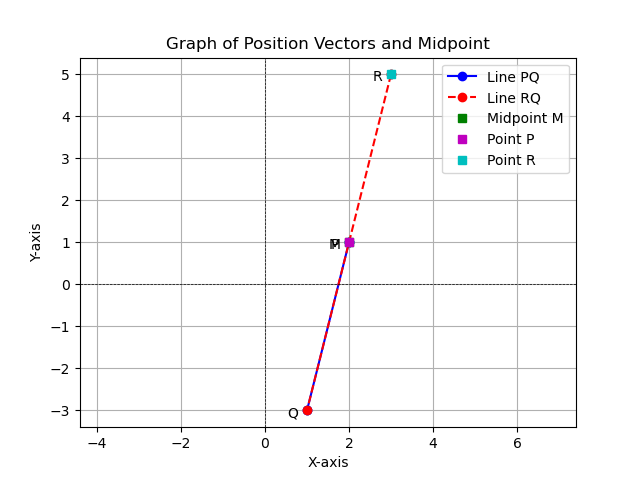
\includegraphics[width=0.7\linewidth]{figs/graph.png}
   \caption{Position Vector Division}
\end{figure}
\end{document}
